\subsection{Drivetrain}\label{DriveTrain}
The drivetrain translates the torque $\tau_m$, given by the motor, into the actual movement of the vehicle. A mechanical depiction of the parts considered in this modeling section can be seen on \figref{fig:DrivetrainMechanicalModel}. Here the input torque to the system, given by the motor shaft, translates through the system ending up as a linear velocity of the vehicles mass on the belts, i.e. the velocity of the vehicle. The velocity model of the drivetrain is created by only considering when the vehicle's trajectory follows a straight line.\\\\

\begin{figure}[H]
	\centering
	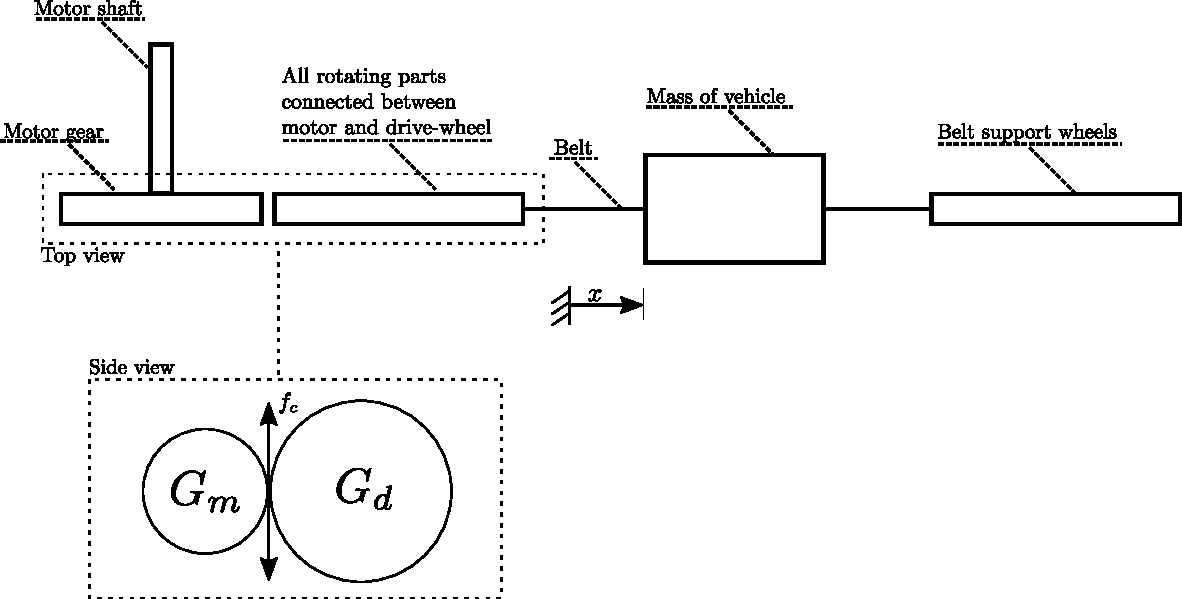
\includegraphics[scale=0.8]{figures/mechanicalDrawingSystem.pdf}
	\caption{A diagram showing the outlines of the mechanical model of the drivetrain}
	\label{fig:DrivetrainMechanicalModel}
\end{figure}

To make it more manageable the modeling of the drivetrain is limited to only modeling parts of the total drivetrain system.

\subsubsection{Model of the Internal Gears}\label{BlackBoxModel}
To get a rough approximation of the effect of the drivetrain, a black boxed model is used. The black box in the model is placed between box 1 and including box 3 seen in \chapref{sec:Vehicledescription} \figref{vehicleDescriptionDriveTrain}. The gear, $G_m$, connected to the motor shaft, is connected to the gear, $G_d$, which represents the gears and shafts that has been black boxed. The output of black box is given on the shaft connected to the drive-wheel, $G_t$, see \figref{fig:DrivetrainMechanicalModel}. The number of teeth on the gear, $G_d$, represents the gear ratios throughout the drivetrain, such that the gear ratio between $G_m$ and the output at the drive gear is given by: $\frac{N_m}{N_d}$, where $N_m$ is the number of teeth on the motor gear and $N_d$ is the calculated number of teeth on the black box gear.

The torque of the motor along with the contributions from the load, i.e. the drivetrain, affecting the motor shaft, is depicted in as a free body diagram in \figref{fig:MotorGearFreeBodyDiagram}.

\begin{figure}[H]
	\centering
	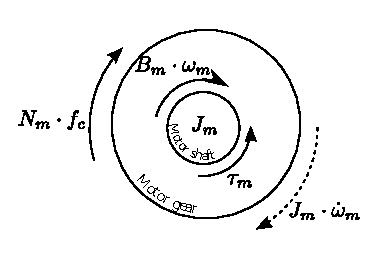
\includegraphics[scale=1.2]{figures/freeBodyMotorGear.pdf}
	\caption{A free body diagram of the motor gear, $G_m$}
	\label{fig:MotorGearFreeBodyDiagram}
\end{figure}

The radius of the motor gear times the contact force, $r_m \cdot f_c$, is the torque translated from the motor gear, $G_m$, to the gear representing the drivetrain, $G_d$, in \figref{fig:BlackBoxGearFreeBodyDiagram}. Thus it appears as an opposing torque to the applied motor torque, $\tau_m$. From \figref{fig:MotorGearFreeBodyDiagram}, the following equation can be derived:
 \begin{flalign}
   \eq{J_m \cdot \dot{\omega}_m(t)} {\tau_m(t) - B_m \cdot \omega_m(t) - r_m \cdot f_c(t)}\unit{N \cdot m}\nonumber
   \label{eq:MotorGearNewtonSecLaw}
 \end{flalign}
%
\hspace{6mm} Where:\\
\begin{tabular}{ p{1cm} l l l}
& $J_m$ 						& is the motor's inertia                                         &\unitWh{kg \cdot m^2} \\
& $\omega_m$        & is the angular velocity of the motor                           &\unitWh{rad \cdot s^{-1}} \\
& $\dot{\omega}_m$ 	& is the angular acceleration of the motor                       &\unitWh{rad \cdot s^{-2}} \\
& $\tau_m$ 			    & is the torque delivered by the motor                           &\unitWh{N \cdot m} \\
& $B_m$             & is the motor's friction coefficient                            &\unitWh{N \cdot m \cdot s \cdot rad^{-1}} \\
& $r_m$             & is the radius of the gear, $G_m$, connected to the motor shaft &\unitWh{m} \\
& $f_c$							& is the contact force between the two gears                     &\unitWh{N}
\end{tabular}

To find the output of the drivetrain, a free body diagram is developed and illustrated in \figref{fig:BlackBoxGearFreeBodyDiagram}. The figure represents the system's effecting torques on the blackbox gear, $G_d$, and the translation of these to the drive wheel.

\begin{figure}[H]
	\centering
	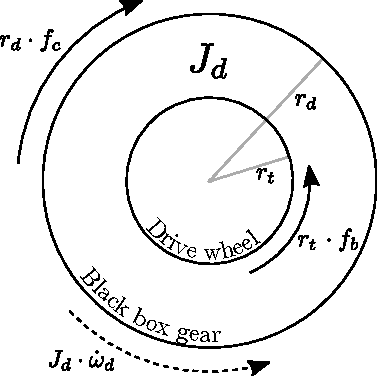
\includegraphics[scale=1]{figures/freeBodyDriveGear.pdf}
	\caption{A free body diagram of the `black box' gear, $G_d$}
	\label{fig:BlackBoxGearFreeBodyDiagram}
\end{figure}

An equation is extracted from \figref{fig:BlackBoxGearFreeBodyDiagram}:
\begin{flalign}
\eq{J_d \cdot \dot{\omega}_d(t)}{r_d \cdot f_c(t) - r_t \cdot f_b(t)} \unit{N\cdot m}
\label{eq:BlackBoxGearNewtonSecLaw}
\end{flalign}
\hspace{6mm} Where:\\
\begin{tabular}{p{1cm}lll}
& $J_d$ 						& is the `black box' gear inertia                                    &\unitWh{kg \cdot m^2} \\
& $\dot{\omega}_d$ 	& is the angular acceleration of the `black box' gear, $G_d$         &\unitWh{rad \cdot s^{-2}} \\
& $r_d$             & is the radius of the `black box' gear, $G_d$                       &\unitWh{m} \\
& $r_t$             & is the radius of the drive wheel, $G_t$ (translational)            &\unitWh{m} \\
& $f_b$             & is the coefficient of the contact force between $G_d$ and the belt &\unitWh{N} \\
& $f_c$						  & is the contact force between the two gears                         &\unitWh{N}
\end{tabular}

Two equations for the internal gears have been found, \eqref{eq:MotorGearNewtonSecLaw} and \eqref{eq:BlackBoxGearNewtonSecLaw}. In the following paragraph a model of the translation between the drive-gear and the belt is created.

%% SSSECTION : BELT MODEL %%
\subsubsection{Translational Model}\label{BeltModel}
It is necessary to find the translation between the drive-gear and the belt to be able to describe the movement of the vehicle. Furthermore, it is needed to be able to make a full model of the system, going from the gear connected to the motor shaft to the vehicle's belts. In \figref{fig:BeltMechanicalDiagram} a mechanical diagram illustrates how the force, given through the drive wheel, is translated by the belts. The translation yields a linear force acting on the mass, which makes the vehicle move with a corresponding velocity.

\begin{figure}[H]
	\centering
	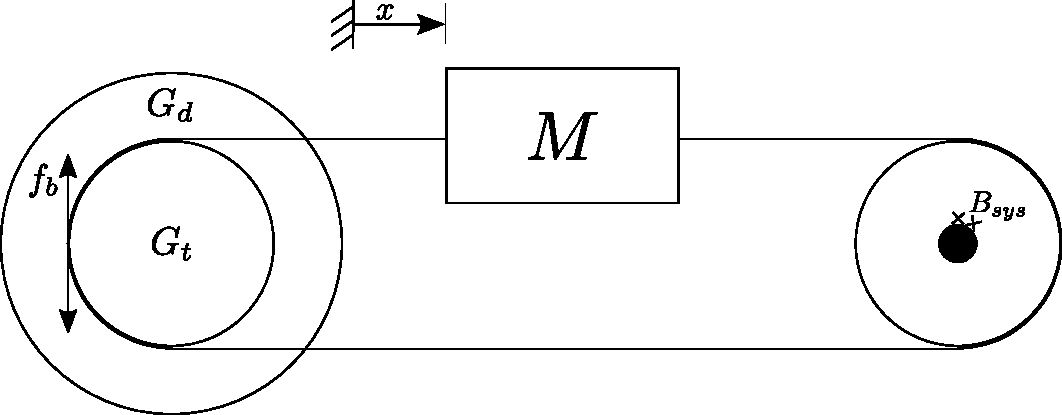
\includegraphics[scale=0.8]{figures/mechanicalDrawingBelt.pdf}
	\caption{A mechanical diagram of the drive-gear rotating the belt affected by the vehicle's mass}
	\label{fig:BeltMechanicalDiagram}
\end{figure}

By using \figref{fig:BeltMechanicalDiagram} a free body diagram of the mass, $M$, and the forces applied to the mass is derived.

\begin{figure}[H]
	\centering
	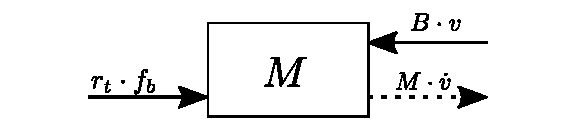
\includegraphics[scale=.8]{figures/freeBodyBelt.pdf}
	\caption{A free body diagram illustrating the vehicle's mass affected by the surrounding forces}
	\label{fig:BeltFreeBodyDiagram}
\end{figure}

From \figref{fig:BeltFreeBodyDiagram}, a mechanical equation of the vehicle's resulting force is found to be:
%
\begin{flalign}
\eq{M \cdot \dot{v}(t)}{f_b(t) - B_{sys} \cdot v(t)} \unit{N}
\label{eq:BeltMassNewtonSecLaw}
\end{flalign}
\hspace{6mm} Where:\\
\begin{tabular}{p{1cm}lll}
& $M$ 			  & is the vehicle's total weight                                        &\unitWh{kg} \\
& $v$        	& is the linear velocity of the vehicle                                &\unitWh{m \cdot s^{-1}} \\
& $\dot{v}$ 	& is the linear acceleration of the vehicle                            &\unitWh{m \cdot s^{-2}} \\
& $B_{sys}$   & is the coefficient of the friction throughout the rotational parts   &\unitWh{N \cdot s \cdot m^{-1}} \\
\end{tabular}

In the following section the three mechanical equations, \eqref{eq:MotorGearNewtonSecLaw}, \eqref{eq:BlackBoxGearNewtonSecLaw1} and \eqref{eq:BeltMassNewtonSecLaw} is combined.

\subsubsection{Model of the Combined Drivetrain}\label{DrivetrainModeling}
In this section a model will be created of the combined drivetrain, by assembling the derived mechanical equations, \eqref{eq:MotorGearNewtonSecLaw}, \eqref{eq:BlackBoxGearNewtonSecLaw1} and \eqref{eq:BeltMassNewtonSecLaw}. This allows to get a linear velocity of the vehicle, \si{V(s)}, from the torque, \si{\tau_m}, delivered by the motor. The three equations are linked through the contact forces \si{f_c} and \si{f_b}.\\\\
%
The Laplace-transform is applied on the three equations in order to deduce a transfer function of the input torque, \si{\tau_m(s)}, to the output velocity, \si{V(s)}:
%
\begin{flalign}
\eq{J_m \cdot \omega_m(s) \cdot s}{\tau_m(s) - B_m \cdot \omega_m(s) - r_m \cdot F_c(s)}&
\label{eq:MotorGearNewtonSecLawLaplace}
\end{flalign}
%
\begin{flalign}
\eq{J_d \cdot \omega_d(s) \cdot s}{r_d \cdot F_c(s) - r_t \cdot F_b(s)}&
\label{eq:BlackBoxGearNewtonSecLawLaplace}
\end{flalign}
%
\begin{flalign}
\eq{M \cdot V(s) \cdot s}{F_b(s) - B_{sys} \cdot V(s)}&
\label{eq:BeltMassNewtonSecLawLaplace}
\end{flalign}

\si{F_c(s)} is isolated from \eqref{eq:MotorGearNewtonSecLawLaplace}:
\begin{flalign}
\eq{F_c(s)}{\frac{\tau_m(s) - B_m \cdot \omega_m(s) - J_m \cdot \omega_m(s) \cdot s}{r_m}}&
\label{eq:GearsContactForceMotorGearLaplace}
\end{flalign}
%
\si{F_b(s)} is isolated from \eqref{eq:BlackBoxGearNewtonSecLawLaplace}:
\begin{flalign}
\eq{F_b(s)}{\frac{r_d \cdot F_c(s) - J_d \cdot \omega_d(s) \cdot s}{r_t}}&
\label{eq:GearsContactForceBlackBoxGearLaplace}
\end{flalign}
%
\si{F_b(s)} is isolated from \eqref{eq:BeltMassNewtonSecLawLaplace}.
\begin{flalign}
\eq{F_b(s)}{V(s) \cdot (M \cdot s - B_{sys})}&
\label{eq:BeltContactForceLaplace}
\end{flalign}

The \si{F_c(s)} in \eqref{eq:GearsContactForceBlackBoxGearLaplace} is substituted for the expression given by \eqref{eq:GearsContactForceMotorGearLaplace}:
\begin{flalign}
\eq{F_b(s)}{\frac{r_d \cdot (\frac{\tau_m(s) - B_m \cdot \omega_m(s) - J_m \cdot \omega_m(s) \cdot s}{r_m}) - J_d \cdot \omega_d(s) \cdot s}{r_t}}&\nonumber\\
\eq{F_b(s)}{\frac{\tau_m(s) \cdot r_d}{r_m\cdot r_t} - \frac{\omega_m(s)\cdot r_d}{r_m\cdot r_t}\cdot (B_m + J_m \cdot s) - \frac{\omega_d(s)}{r_t}\cdot J_d\cdot s}&
\label{eq:BlackBoxGearNewtonSecLawLaplace&MotorGearNewtonSecLawLaplace}
\end{flalign}

The two expressions for \si{F_b(s)}, \eqref{eq:BlackBoxGearNewtonSecLawLaplace&MotorGearNewtonSecLawLaplace} and \eqref{eq:BeltContactForceLaplace}, are coupled:
\begin{flalign}
\eq{V(s) \cdot (M \cdot s - B_{sys})}{\frac{\tau_m(s) \cdot r_d}{r_m\cdot r_t} - \frac{\omega_m(s)\cdot r_d}{r_m\cdot r_t}\cdot (B_m + J_m \cdot s) - \frac{\omega_d(s)}{r_t}\cdot J_d\cdot s}&
\label{eq:BlackBoxGearNewtonSecLawLaplace&MotorGearNewtonSecLawLaplace&&BeltContactForceLaplace}
\end{flalign}

By using the relationship of ratios, the two rotational velocities are related. This is done as a step towards converting all rotational velocities to linear velocities.
\begin{flalign}
\eq{\frac{r_m}{r_d}}{\frac{\omega_d(t)}{\omega_m(t)}}\nonumber \unit{\cdot}\\
\eq{\omega_d(t)}{\frac{r_m}{r_d}\cdot \omega_m(t)} \unit{rad\cdot s^{-1}}
\label{eq:ratioes}
\end{flalign}

$\omega_d(t)$ is converted to a linear velocity and transformed to the Laplace domain:
\begin{flalign}
\eq{v(t)}{\omega_d(t) \cdot 2 \cdot \pi \cdot r_t}\nonumber \unit{m\cdot s^{-1}} \phantom{(3.23   3)}\\
\eq{\omega_d(t)}{\frac{v(t)}{2\cdot \pi \cdot r_t}} \ \xRightarrow{\mathcal{L}} \ \omega_d(s) = \frac{V(s)}{2\cdot \pi \cdot r_t}&
\label{eq:omegaDtoLinearLaplace}
\end{flalign}

$\omega_m(t)$ is converted to a linear velocity using \eqref{eq:ratioes} and \eqref{eq:omegaDtoLinearLaplace} and transformed to the Laplace domain
\begin{flalign}
\eq{\frac{r_m}{r_d}\cdot \omega_m(t)}{\frac{v(t)}{2\cdot \pi \cdot r_t}}\nonumber \unit{rad\cdot s^{-1}} \phantom{(3.23   3)}\\
\eq{\omega_m(t)}{\frac{v(t)\cdot r_d}{2\cdot \pi \cdot r_t\cdot r_m}}  \ \xRightarrow{\mathcal{L}} \ \omega_m(s) = \frac{V(s)\cdot r_d}{2\cdot \pi \cdot r_t\cdot r_m}
\label{eq:omegaMtoLinearLaplace}
\end{flalign}

Using the previously derived equations, \eqref{eq:BlackBoxGearNewtonSecLawLaplace&MotorGearNewtonSecLawLaplace&&BeltContactForceLaplace}, \eqref{eq:omegaDtoLinearLaplace} and \eqref{eq:omegaMtoLinearLaplace}, the final transfer function, describing the drivetrain, including the mechanical aspect from the motor, is constructed:

\begin{flalign}
\eq{V(s) \cdot (M \cdot s - B_{sys})}{\frac{\tau_m(s) \cdot r_d}{r_m\cdot r_t} - \frac{\frac{V(s)\cdot r_d}{2\cdot \pi \cdot r_t\cdot r_m}\cdot r_d}{r_m\cdot r_t}\cdot (B_m + J_m \cdot s) - \frac{\frac{V(s)}{2\cdot \pi \cdot r_t}}{r_t}\cdot J_d\cdot s}&\nonumber\\
\eq{\frac{V(s)}{\tau_m(s)}}{\frac{\frac{1}{ \frac{r_m\cdot r_t}{r_d} \cdot B_{sys} + \frac{r_d}{2\cdot \pi \cdot r_m \cdot r_t} \cdot B_m }}{\frac{ \frac{r_m\cdot r_t}{r_d} \cdot M + \frac{r_d}{2\cdot \pi \cdot r_m \cdot r_t} \cdot J_m + \frac{r_m}{2\cdot \pi \cdot r_t \cdot r_d} \cdot J_d }{\frac{r_m\cdot r_t}{r_d} \cdot B_{sys} + \frac{r_d}{2\cdot \pi r_tm \cdot r_t} \cdot B_m} \cdot s + 1}}\label{eq:mechanicalTransFerfunction}
\end{flalign}

The mechanical part of the system is described by the above transfer function, \eqref{eq:mechanicalTransFerfunction}, which in the following section is used in collaboration with the electrical model of the motor to describe the full velocity model of the vehicle.